
% Background and Significance
% No page limit
\chapter{Multivariate Analysis of Thalamo-Cortical Structural Connectivity Loss in TBI}
\label{chap_tbi}

This chapter presents work that was presented at the Computer Vision and Pattern Recognition workshop on Mathematical Methods in Biomedical Image Analysis 2008, Anchorage, AK~\cite{duda08mmbia}. The technical aspects of the multivariate registration were completed in collaboration with Brian Avants and are discussed in greater detail in two works on which I am second author, a  manuscript that appeared in Academic Radiology~\cite{Avants2008} and work presented at the 10th International Conference on Medical Image Computing and Computer Assisted Intervention 2007, Brisbane, Australia~\cite{Avants2007}. Diffusion tensor images (DTI) quantify connectivity patterns in the brain while the T1 modality provides high-resolution images of tissue interfaces.  Our objective was to use both modalities to build subject-specific, quantitative models of fiber connections in order to discover effects specific to a neural system. The health of the thalamo-cortical network is compromised by traumatic brain injury, and we hypothesized that these effects are due to a primary injury to the thalamus which results in subsequent compromise of radiating fibers. We first used a population-specific average T1 and DT template to label the thalamus and Brodmann areas (BA) 9,10 and 11 in each subject.  We also built an expected connection model within this template space that was transferred to subject-space in order to provide a prior restriction on probabilistic tracking performed in subject space.  We evaluated the effect of traumatic brain injury on this prefrontal-thalamus network by quantifying, in 10 subjects and 8 controls, the mean diffusion and fractional anisotropy (FA) along fiber tracts, along with the mean diffusion within the thalamus and cortical regions.  We contrasted results gained by a template-based tract definition with those gained by performing analysis in the subject space. Both approaches revealed connectivity structural effects of TBI, specifically a region of reduced FA in the white matter connecting the thalamus to BA 10. 

%%%%%%%%% BODY TEXT
\section{Introduction}
Traumatic brain injury (TBI) is the most frequent cause of death and disability in individuals ages 15 to 24 and is also prevalent in older adults~\cite{Furlow2006}. TBI, most commonly caused by automotive accidents and falls, occurs at a rate of approximately 1 in 600 per year in the general population~\cite{Furlow2006}, whereas up to 10\% of soldiers returning from Iraq may suffer from some form of TBI~\cite{Hoge2008}. Even mild TBI may lead to significant behavioral changes~\cite{Kraus2007} and is very likely to be under-reported, particularly by those who have experienced concussion~\cite{Mendez2005,Chen2008}. In consequence, up to 2\% of individuals in the United States live with TBI-related disability. Thus, focus on TBI as a public health concern is increasing, along with further development of sensitive tools for assessing axonal and cortical injury~\cite{Kraus2007,Kim2008}, tracking recovery from these injuries~\cite{Levin2003} and predicting outcome~\cite{Miles2008,Sidaros2008}.

Traditional T1 imaging may be used to uncover in vivo effects of TBI in the cortex and deep gray matter structures. Neuronal atrophy, from concussion, was detected with T1 imaging and linked to ongoing depression~\cite{Chen2008}, whereas TBI-related reductions in gray matter concentration have also been correlated with attention deficits~\cite{Gale2005}. Hippocampal volume may be reduced by TBI~\cite{Tomaiuolo2004,Salmond2005}, along with the basal forebrain~\cite{Salmond2005}. The thalamus appears to undergo injury during or after TBI as assessed postmortem~\cite{Graham2005}, through finite element models of TBI~\cite{Mendez2005,Zhang2004} and through large-deformation tensor-based morphometry of control and subject populations~\cite{Kim2008}. An additional postmortem report has indicated involvement of the mediodorsal thalamus, which has connections to the pre-frontal cortex~\cite{Maxwell2004}. This finding has also been validated at the cellular level through neuropathology~\cite{Adams2000} and through histochemical staining and explicit neuronal counts~\cite{Maxwell2006}. TBI effects in the hippocampus have also been verified neuropathologically~\cite{Ahn2006}.

Despite the value of T1 imaging for examining cortical atrophy, increasing evidence suggests that traditional magnetic resonance imaging has limited ability to detect TBI-related damage outside the cortex or deep gray matter, where diffusion tensor imaging (DTI) may be more valuable~\cite{Ahn2006,Bazarian2007,Donald2007a,Lee2006}. During TBI, acceleration of the head results in mechanical forces that compress frontal regions and stretch posterior regions~\cite{Bayly2005}. These forces result in microstructural damage to brain tissue, known as diffuse axonal injury (DAI). Immediately after TBI, the microstructural effects of DAI manifest as disruptions in the cytoskeletal network and axonal membranes~\cite{Arfanakis2002,Benson2007,Liu1999}. This results in the formation of axonal `retraction balls' which are thought to be a consequence of axoplasm accumulation~\cite{Bullock2005}. This is followed by axonal disconnection. Pathological examinations of DAI have suggested that small hemorrhages often accompany DAI~\cite{Scheid2007}. Changes in diffusion are hypothesized to relate to axonal swelling in TBI~\cite{Bazarian2007} or myelin loss~\cite{Song2002}. Thus, DTI is emerging as the preferred mechanism for revealing traumatic axonal injury through a variety of diffusion-related measures. 

Studies have analyzed DTI-based metrics to show that TBI leads to strong effects in the corpus callosum~\cite{Levin2000,Ewing-Cobbs2006,hashimoto2007,Inglese2005,Nakayama2006,Xu2007,Kumar2009,Lipton2008,Miles2008,Rutgers2008,Sidaros2008,Takayama2000,Voss2006}, which may imply a disruption of brain connectivity~\cite{Sugiyama2007,Le2005}. Brain regions related to motor function are also affected~\cite{Lee2006,Yasokawa2007}, but may also recover over time~\cite{Han2007}. White matter pathology caused by TBI may also appear in a number of fascicles and may lead to cognitive deficits~\cite{Kraus2007}. A few studies have suggested that mean diffusion implies cortical injury or pathology~\cite{Ardekani2005,Kantarci2001,Chappell2006}. Increases in mean diffusion from mild cognitive impairment (MCI) have been directly related to reductions in cognitive performance~\cite{Ray2006}. Only two DTI studies have shown evidence of thalamic injury~\cite{Salmond2006,Avants2008}, despite the ability of DTI imaging to detect the subdivisions of thalamus into its nuclei~\cite{Duan2007,Wiegell2003}. Such divisions are not visible in T1.

Major depressive disorder (MDD) often results from mild TBI and negatively impacts psychosocial function and cognitive performance~\cite{Fann1997,Feinstein2006,Jorge2004}. Post-TBI major depression inhibits recovery~\cite{Gordon2006b,Jorge2005} and, while variable, may occur in as many as 77\% of patients~\cite{Alfano2006,Ashman2004,Deb1999,Jorge2005,Reekum2000}. Evidence has linked the structural changes in the prefrontal cortex to both TBI~\cite{Jorge2004} and depression~\cite{Koenigs2008}. Additionally, structural changes in the thalamus have also been linked to TBI~\cite{Graham2005} and depression~\cite{Young2004}. The functional links between depression and TBI and the implication of structural changes in the prefrontal cortex and thalamus in both disorders, suggests the possible influence of DAI in the thalamo-cortical network. Here we used a multivariate atlas to identify the prefrontal components of the thalamo-cortical network in order to examine the structural properties of the prefrontal cortex, the thalamus, and the white matter pathways that connects them.

% Alt Intro
%Traumatic brain injury (TBI) is the most frequent cause of death and disability in individuals under age 40 in the industrialized world~\cite{Furlow2006}.  Even mild TBI may lead to long-term behavioral consequences~\cite{King1997,Kraus2007} that often involve deficits in executive functioning~\cite{Wozniak2007}.  Thus, TBI is a major epidemiological concern~\cite{Furlow2006,Hoge2008}.

%Evidence is emerging that multiple modality studies are particularly effective in monitoring TBI~\cite{Ibrahim2007}.  Traditional T1 imaging may be used to uncover {\em in vivo} effects of TBI in the cortex and deep gray matter structures~\cite{Chen2008,Gale2005,Salmond2005}. Post-mortem~\cite{Graham2005}, simulation~\cite{Mendez2005,Zhang2004} and large-deformation tensor-based morphometry studies~\cite{Kim2008} indicate that thalamus, which has prominent connections to the prefrontal cortex~\cite{Maxwell2004}, is commonly affected by TBI. While T1 imaging is of great value, diffusion tensor imaging is equally important for its complementary measures of white matter integrity through fractional anisotropy (FA)~\cite{Ahn2006,Bazarian2007,Donald2007} and gray matter integrity through mean diffusion (MD)~\cite{Song2002,Mori2006}. Voxel-based DT studies have analyzed these diffusion-related measures to show that TBI leads to strong effects in the corpus callosum~\cite{Levin2000,Ewing-Cobbs2006,Hashimoto2007} while fiber-based analyses have shown evidence of tract interruptions~\cite{Naganawa2004}.  However, only one DT study has shown evidence of thalamic injury~\cite{Salmond2006} and few perform any analysis outside white matter.  

%The use of DTI in tract based studies has received much attention recently~\cite{Corouge2006,Ding2003,Jones2005,Fillard2003} and the TBSS method~\cite{Smith2006} has proven to be particularly useful in whole-brain analysis of FA. Here the focus in on a particular neural system that includes both gray matter and white matter structures. Multivariate methods are used to create a model of this system by exploiting the data most relevant to particular structures in an effort to gain further insight into the complex effects of traumatic brain injury.

%------------------------------------------------------------------------
\section{Materials and Methods}

Our approach extended previous DTI and T1-based studies by building an explicit multivariate model of an important network that connects the limbic thalamus with the frontal lobes responsible for executive function, planning and motivation~\cite{Cummings1993}. This model was used to identify the particular cortical regions to which thalamic connections are compromised.
The use of a multivariate image normalization method provided a population specific atlas. The DTI component of the atlas was used for fiber tractography. Tracts between the thalamus and three subregions of the frontal cortex were identified and used to create model connection paths. These models were transformed to each individual where probabilistic tractography was performed. The models were then used as a prior for examining the individual's tractography to obtain a subject-specific connection with a common frame-of-reference that facilitates inter-subject comparison of FA and MD. The MD in the cortex and thalamus was also examined in order to gain insight into system-wide effects of TBI. This process is outlined in figure \ref{fig:process}.

\begin{figure*}
\center{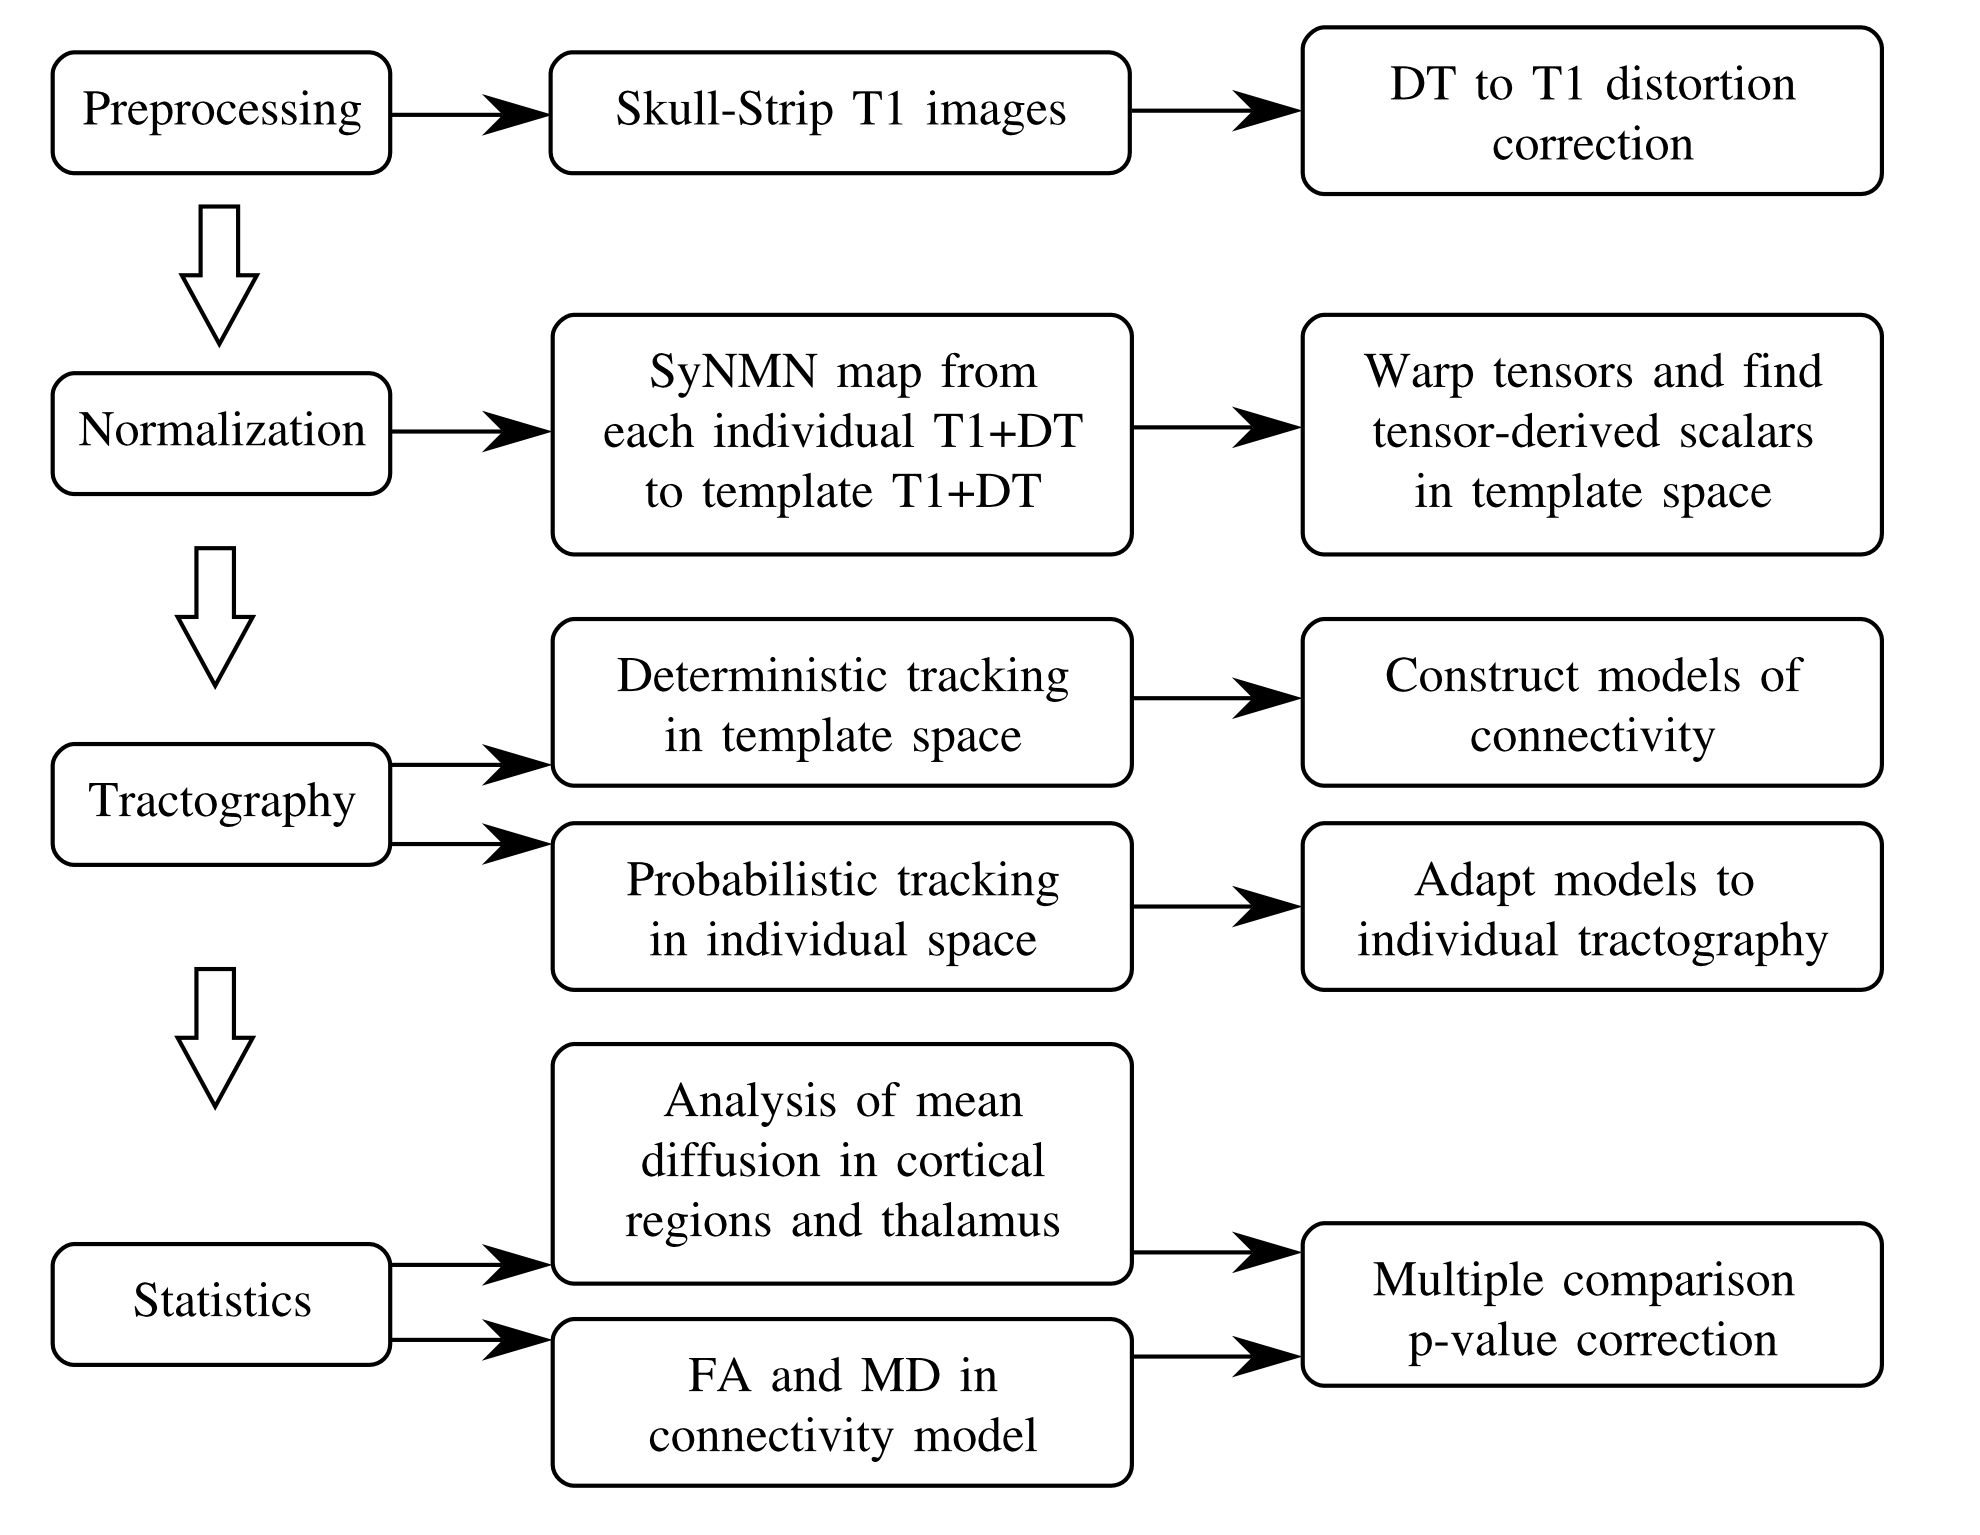
\includegraphics[width=0.9\linewidth]{figures/process.png}}
\caption{A overview of the steps required in the processing for
the population analysis of structure and connectivity.}
\label{fig:process}
\end{figure*}

\subsection{Cohort and Image Dataset}
The data was collected as part of a larger study investigating the neural correlates of attention deficits and treatment responses of
various psychoactive drugs in the survivors of TBI.  Our cohort included 10 individuals with TBI and 8 healthy controls. The 10 subjects with TBI included 6 men and 4 women aged between 21 and 59 years (mean age = 35.0, SD = 12.1) with a mean education of 13.3 years (SD = 1.7).  Control participants included 5 men and 3 women aged between 23 and 46 years (mean age = 36.2, SD = 8.8) with a mean education of 14.5 years (SD = 2.0).  The two groups did not differ significantly in terms of age, gender, ethnicity, handedness or years of education (tested with t-test or Fisher's exact test, as appropriate).

\subsubsection{Imaging parameters}
DT images were collected with a single-shot, spin-echo, diffusion-weighted echo-planar imaging (EPI) sequence and a GRAPPA parallel imaging acquisition.  The diffusion sampling scheme consisted of one image without diffusion gradients (b=0s/mm$^2$), followed by 30
non-collinear and non-coplanar diffusion encoding directions isotropically distributed in space (b=1000s / mm$^2$).  Additional imaging parameters were: TR=7300ms, TE=91ms, number of averages=1, and 1.875 mm$^2$ in-plane and 2mm out-of-plane resolution. High resolution T1-weighted anatomic images were obtained using 3D MPRAGE imaging sequence and the following acquisition parameters: TR = 1620 ms, TI = 950 ms, TE = 3 ms, flip angle = 15 degrees, 160 contiguous slices of 1.0 mm thickness, FOV = 192 $\times$ 256 mm$^2$, matrix = 192 $\times$ 256, 1NEX with a scan time of 6 min. The resulting voxel size was 1 mm$^3$.  All T1 images were skull-stripped by using symmetric normalization (SyN)~\cite{Avants2008} to map a brain mask from a template to each individual image.

\subsection{Normalization}
First an intra-subject, small deformation registration is performed with SyN, a univariate version of SyNMN, between each subject's T1 and FA images in order to correct for potential misalignment and distortion. The use of symmetric normalization techniques is particularly useful when working with both images and fiber tractography.  Image data is typically warped ``backward'' while point-based objects such as fibers are more easily warped ``forward'' using the inverse transform. Utilizing a method that inherently provides this symmetric mapping eliminates the need for {\em ad hoc} approaches for guaranteeing the invertibility of the transforms.
The normalization provided by SyNMN minimizes an energy function consisting of an image similarity term, $D_{sim}$, and a transformation metric distance term, $D_{shape}$, within the space of diffeomorphisms. This produces a series of maps, $\phi(x,t)$, that smoothly deform image $I$ into the space of image $J$ and, at the end point, $\phi(x,1.0)$, minimizes the following energy,

\begin{equation}
D_{shape}^2(\phi(x,0),\phi(x,1)) + D_{sim}(\phi(x,1),I,J)
\end {equation}

In order to examine both T1 and DT simultaneously, $D_{sim}$ is the weighted sum of two terms:
\begin{eqnarray}
D_{sim}(I,J,\phi) =& \omega_1(x)MI(I_{T1}(\phi_1),J_{T1}(\phi_2)) + \nonumber \\ &  \omega_2(x)\Vert(I_{DT}(\phi_1) - J_{DT}(\phi_2))\Vert_{DV}^2
\end{eqnarray}
where $MI$ is the mutual information and $\Vert(D_1 - D_2))\Vert_{DV}$ is the {\em deviatoric} Euclidean distance between two diffusion tensors~\cite{Alexander99}. Spatially varying weights are chosen to emphasize the tensor data in areas where the FA is high and prioritize the T1 data elsewhere. Additionally, it is desired that the weighting function be smooth. The first term of the weighting is given as $\omega_1 = G_{\sigma} \star (1.0 - FA(x))$ where $FA(x)$ is the 0.25 thresholded FA image and $G_{\sigma}$ is a Gaussian smoothing kernel operating on the weight function. The weights are constrained to sum to one so $\omega_2 = 1.0 - \omega_1$. The gradients of these terms are used to determine a mapping between any individual and a template using a standard multi-resolution gradient descent strategy. At each iteration, the DTI components are reoriented using the preservation of principal direction formulation~\cite{Alexander01}. Figure \ref{fig:atlas} illustrates the template provided by this technique. To examine the structural integrity of the cortical regions and thalamus, MD is examined at each point with a Student's t-test. We only consider results with an FDR-corrected p-value $<$ 0.02 and with a cluster size of at least 15 voxels.

\begin{figure}
\center{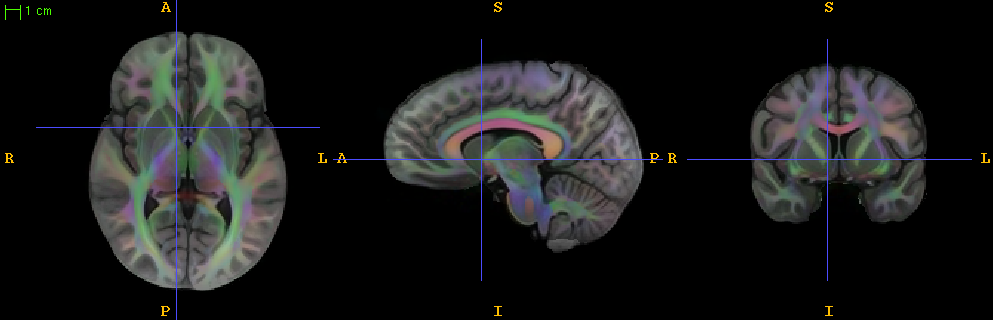
\includegraphics[width=1.0\linewidth]{figures/young_atlas_triplanar.png}}
\caption{Triplanar view of the combined T1 and DTI template provided by SyNMN. The directionally-encoded color map obtained from the principal direction of diffusion in the DTI data provides an overlay to the T1 data.}
\label{fig:atlas}
\end{figure}

\subsection{Connectivity Model}
In order to exploit both the tissue interface information provided by T1 data and the tissue architectural information provided by DTI, a normalization technique known as symmetric normalization of multivariate neuroanatomy (SyNMN) was used to create a population-specific template~\cite{Avants2007}. The use of a multivariate template is particularly useful when examining both gray and white matter properties. The T1 component of the template allows for the accurate identification of BA's as well as the thalamus. The DTI component provided the white matter orientation information that is essential to elucidating the connective pathways between structures. 

Recently, a number of studies have examined methods for using cortical atlases to label DTI generated fiber tracts according to their corresponding cortical regions. This concept has been used to develop connectivity based segmentations of structures such as the thalamus~\cite{Behrens03} and, more extensively, the corpus callosum~\cite{Styner05,Huang05,Hofer06}. Here a similar approach was used to label fibers but with the goal of developing a model of thalamo-cortical connectivity in the prefrontal lobe. To provide a framework for labeling fiber tracts by their associated cortical regions, the Brodmann area (BA) labels provided with the MNI atlas included as part the MRIcro package~\cite{mricro} were transformed into the atlas space by using SyN on the T1 component of the atlas. The FAST image segmentation package~\cite{Zhang01} was used to segment the T1 component of the template. All labeled voxels that were more than 5mm distant from the outer boundary of the gray-matter were excluded. An expert-knowledge guided manual segmentation of the thalamus was performed in the template using both T1 and DTI data. 
 
The DTI component of the template provided a smooth tensor field that was well suited for identifying white matter tracts that are often difficult to track reliably in subject data due to noise. Large bundles of fibers were found for each thalamus to BA connection and were used to determine a model tract for each connection. Whole-brain deterministic tractography was performed using the Camino Toolkit~\cite{Cook06} where all voxels with an FA greater than 0.15 were used as seed points. A constant step size of 0.3 mm was used along with linear interpolation of the principal direction of diffusion vector field. Fibers were terminated when they entered a voxel with FA less than 0.15 or when local curvature of a fiber exceeded 45 degrees. The segmentation of the thalamus and cortical regions allowed for the extraction of fibers connecting these regions. For the purpose of this study, we limited the fibers to those in the anterior thalamus radiata (ATR) which connect the thalamus to BA's 9,10, and 11.

DTI tractography methods are known to produce a number of false-positive pathways. To exclude these, each fiber bundle was filtered to remove fibers of excessive length as well as fibers whose cortical end points were distant from the average end point location. The remaining fibers were then smoothed with BSplines~\cite{Tustison06} and a curve matching algorithm examined local curvature properties~\cite{Avants2003b} to identify corresponding locations on each fiber. A BSpline was fit to the set of corresponding locations on all fibers to determine a final approximation of the white matter pathway. Finally, the curve matching algorithm was used to match the corresponding models in each hemisphere to ensure a consistent parameterization. The model is illustrated in figure \ref{fig:model}. 

%\begin{figure*}
%\center{\includegraphics[width=0.8\linewidth]{model.png}}
%\caption{Thalamo-cortical connectivity models for the prefrontal lobe are created using deterministic tractograpy in a subject-specific atlas. BA's 9 (blue), 10 (purple) and 11 (pink) are used to label the streamlines that connect each region to the thalamus.  Model connections are visualized as tubes with colors corresponding to their cortical regions. The streamlines used to determine the model connections are shown with complementary colors}
%\label{fig:model}
%\end{figure*}

\begin{figure*}
\begin{center}
$\begin{array}{c}
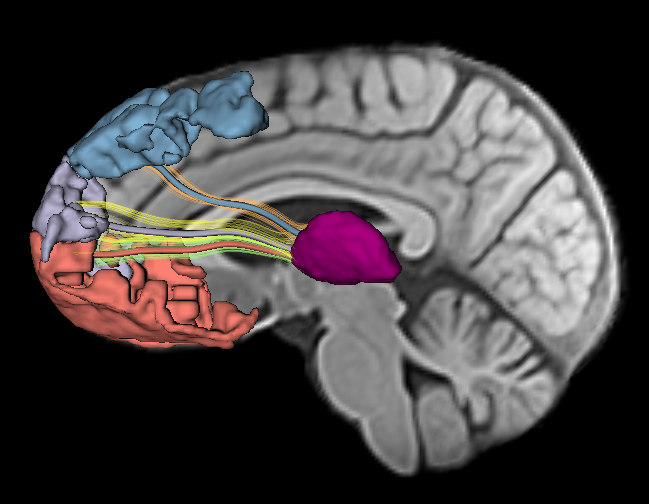
\includegraphics[width=0.75\linewidth]{figures/model1.png} \\
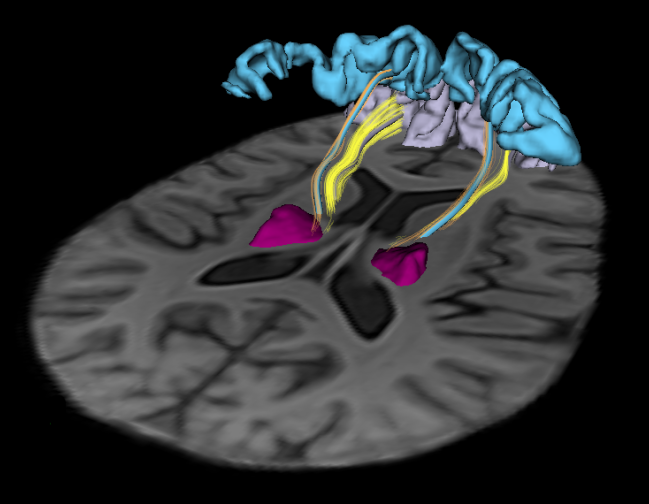
\includegraphics[width=0.75\linewidth]{figures/model2.png}
\end{array}$
\caption{Thalamo-cortical connectivity models for the prefrontal lobe are created using deterministic tractography in a subject-specific atlas. BA's 9 (blue), 10 (purple) and 11 (pink) are used to label the streamlines that connect each region to the thalamus. Model connections are visualized as tubes with colors corresponding to their cortical regions. The streamlines used to determine the model connections are shown with complementary colors.}
\label{fig:model}
\end{center}
\end{figure*}

\subsection{Subject Specific Connectivity Models}
Because the normalization method used does not explicitly match based upon the connectivity between distant structures in the brain it was necessary to identify these pathway in each individuals' DTI data in order to evaluate the usefulness of the template generated model tracts. We warped the model tracts into subject space and used them to search for similar tracts in the probabilistic tractography. This provided a common frame-of-reference for inter-subject comparison while still relying on the tractography obtained from each individual. The transform obtained in the normalization process was used to warp the segmented thalamus and labeled cortical regions in to each individual's native DTI space. All points in the thalamus were used as seed points for wild bootstrapping probabilistic tractography using the Gaussian model of diffusion~\cite{Jones06,Whitcher08}. From each seed point, 1000 fibers were tracked and those that hit labeled cortical regions were retained and labeled. 

Probabilistic tractography methods generate a very large number of tracks which can make processing cumbersome and interpretation difficult. The model tracts were warped into the subject space and served as a framework for determining subject specific model tracts from the probabilistic tractography results. Within each labeled bundle of fibers the mean point-to-point distance between the model tract and each probabilistic tract was used to initially prune the bundle to include the N-closest fibers (N=200). Many of the probabilistic tracts only contained partial segments that were within the specific pathway being examined. This makes the whole-fiber curve matching technique used in the creation of the models unsuitable for use on probabilistic fiber tracts. Instead a point-by-point approach was taken to focus on local properties of the fiber tracts. At each point, $x_m$, in the model the closest point, $x_i$ on each of the N-closest fibers was found, and a weighting was calculated via:
\begin{equation}
\omega_i = e^{\frac{-|x_m - x_i|}{\sigma}}
\end{equation}
The k-highest weights are selected and normalized to sum to one. Here we used $k=40$ and $\sigma=2.0$. A BSpline was used to fit a curve to these weighted points. Additionally, the points and their associated weights were used to calculate a log-Euclidean average tensor at each point~\cite{Arsigny06}. These average tensors were then used to calculate tensor-derived scalars such as FA and MD. Figure \ref{fig:fitting} provides and illustration of the results of the subject specific fitting.

\begin{figure}
\center{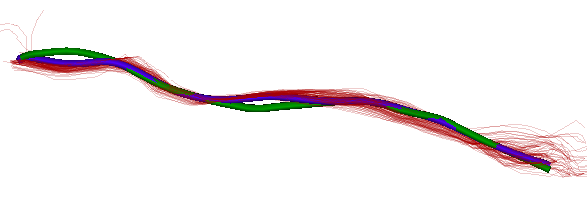
\includegraphics[width=0.75\linewidth]{figures/fitting.png}}
\caption{The connectivity model (green) was warped into the subject space via the transform provided by SyMNM. The results of probabilistic tractography (red) in the individual were then used to adapt to the model to the subject resulting in a model (blue) that more closely represented the subject's anatomy.}
\label{fig:fitting}
\end{figure}

The model tracts were defined in a smooth template space which could reduce their utility in identifying focal differences. In order to evaluate the extent to which this is true, we evaluated a population using both subject-space models and the original model tracts. To do this, we used the model tracts, the template space tractography, and each subject's warped tensor data to determine an average tensor at each point in the tract. When determining the k-closest points, the results of the curve matching obtained in the creation of the model were used to limit the search to the set of corresponding points from each fiber. Otherwise, the process was the same as that taken when using the subject specific tractography. Figure \ref{fig:exconnections} provides an illustration of this technique in both subject-specific and template space. By examining FA and MD along fibers in both the template models and the the subject space models we hoped to gain further insight into each method's ability to identify differences in populations.

\begin{figure*}
\begin{center}
$\begin{array}{ccc}
\textrm{Control} & & \textrm{TBI} \\
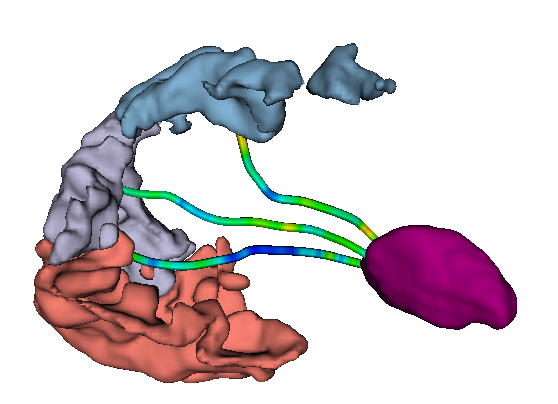
\includegraphics[width=0.4\linewidth]{figures/dc02full.png} & &
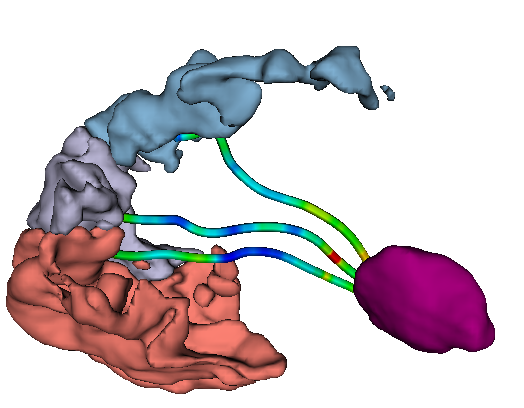
\includegraphics[width=0.4\linewidth]{figures/dp09full.png} \\
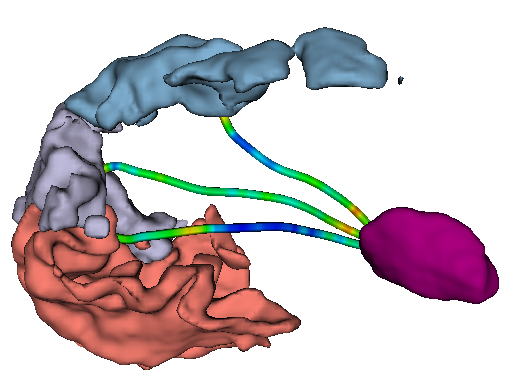
\includegraphics[width=0.4\linewidth]{figures/dc05full.png} & 
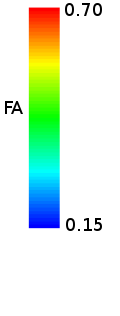
\includegraphics[width=0.1\linewidth]{figures/colorbar.png}&
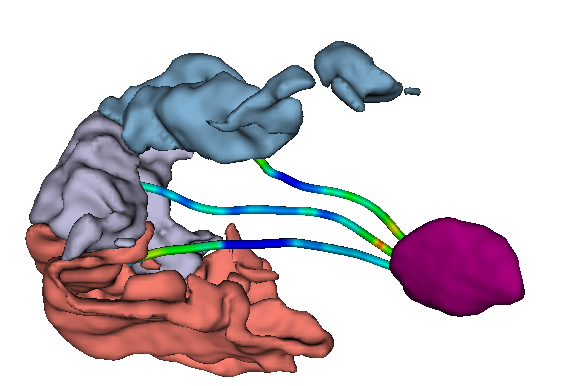
\includegraphics[width=0.4\linewidth]{figures/dp07full.png} \\
 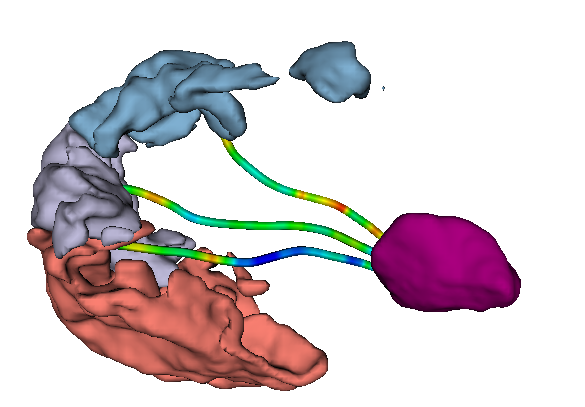
\includegraphics[width=0.4\linewidth]{figures/dc04full.png} & &
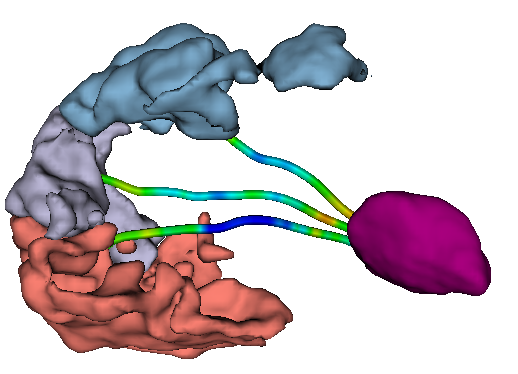
\includegraphics[width=0.4\linewidth]{figures/dp08full.png} \\
\end{array}$
\caption{Subject specific connectivity models for connectivity between thalamus (purple) and BA 9(light blue), 10 (light purple) and BA 11 (pink) are illustrated for three controls (left) and three subjects (right). The connectivity models are colored by average fractional anisotropy.}
\label{fig:exconnections}
\end{center}
\end{figure*}

\section{Results} 
To examine the structural integrity of the cortical regions and thalamus, MD was examined at each point with a Student's t-test. We only considered results with an FDR-corrected p-value $<$ 0.02 and with a cluster size of at least 15 voxels. Compared to controls (N=8), TBI survivors (N=10) showed increased MD in the mediodorsal nucleus of the thalamus~\ref{fig:volstats}. Both the subject-specific and template models were used to examine FA and MD along each connection using a Student's t-test at each point. We only considered results with an FDR corrected p-value $<$ 0.02 and with a 1-D cluster size of at least 5. Figure \ref{fig:connstats} shows the FA differences in the connectivity models of the ATR between control and individuals with TBI as determined by subject-specific connectivity models as well as template space models. In both subject-specific and template space analysis, TBI survivors showed reduced FA near the midpoint of the connection between the thalamus and BA 10 in the left hemisphere. The cluster was located at approximately the same location in each model and is slightly larger in the template space model than in the subject-specific model. The cluster in template space had a maximum t-value of 4.60 while the cluster in the subject-specific analysis had a maximum t-value of 5.26.

\begin{figure}
\begin{center}
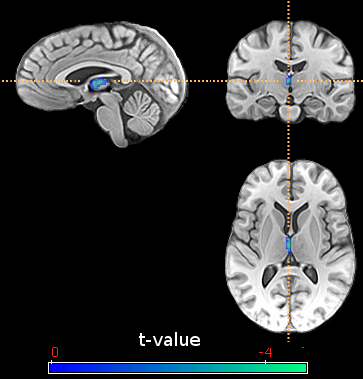
\includegraphics[width=1.0\linewidth]{sigmd.png}
\caption{Mean diffusion is examined in the cortical regions and thalamus. Results with an FDR-corrected p-value $<$ 0.02 and a cluster size of 15 voxels or greater are visualized.}
\label{fig:volstats}
\end{center}
\end{figure}

\begin{figure*}
\begin{center}
\begin{tabular}{ccc}
\multicolumn{3}{c}{Location of fractional anisotropy reduction in TBI} \\
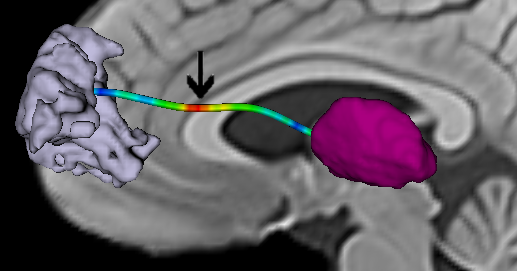
\includegraphics[width=0.42\linewidth]{figures/subject_tstat.png} &
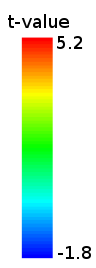
\includegraphics[width=0.08\linewidth]{figures/tcolorbar.png}&
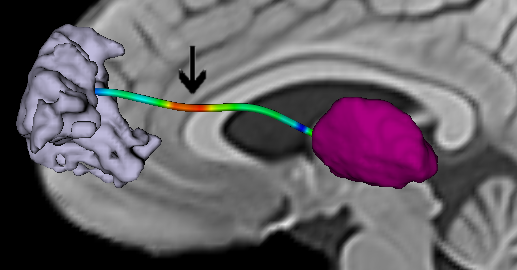
\includegraphics[width=0.42\linewidth]{figures/template_tstat.png} \\
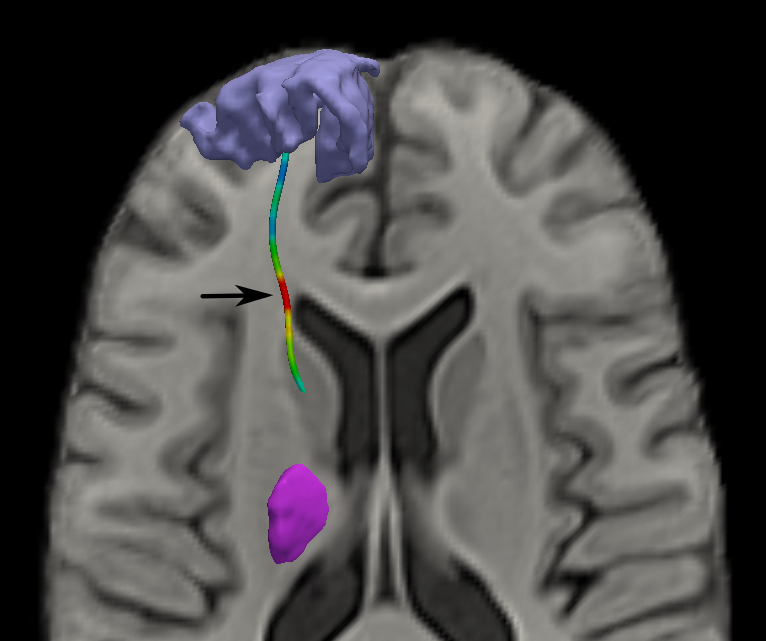
\includegraphics[width=0.42\linewidth]{figures/tbi_subject_axial.png} & &
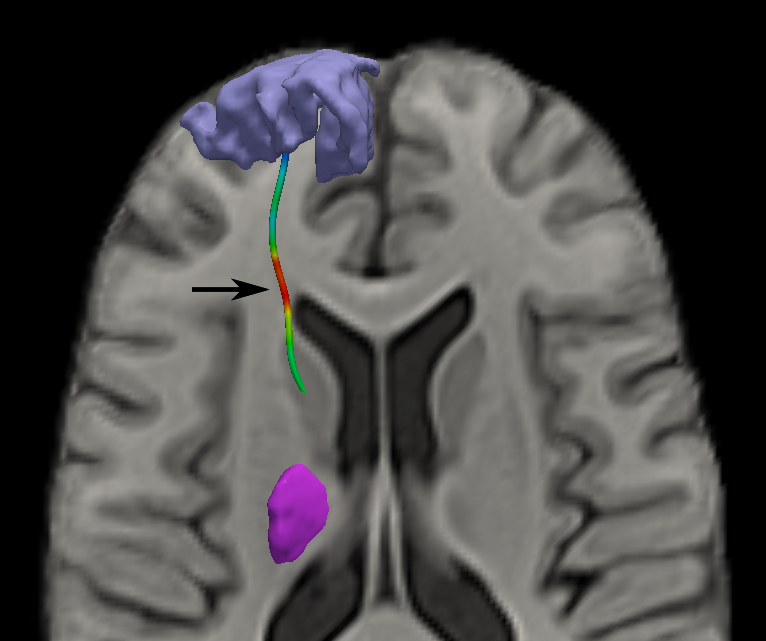
\includegraphics[width=0.42\linewidth]{figures/tbi_template_axial.png} \\
\textrm{Subject space} & & \textrm{Template space} \\
\end{tabular}
\caption{Students t-test results after FDR correction at p$<$0.02 indicated that the left hemisphere connection between thalamus and Brodmann area 10 is affected by TBI. Arrows indicate regions where TBI survivors showed reduced FA compared to controls in both subject space (left) and template space (right) analysis. Sagittal and axial slices from the T1 component of the template are shown for anatomical reference.}
\label{fig:connstats}
\end{center}
\end{figure*}

\section{Discussion}
This study demonstrated that multivariate image registration techniques may be combined with diffusion tensor tractography to create a system-based model for delineating both structural and connective differences in TBI. Localized differences in MD were found in the mediodorsal nucleus of the thalamus. An examination of the white matter fibers that connect this region of the thalamus to the prefrontal cortex revealed significant clusters indicating reduced FA in TBI. The use of a connectivity model that adapts to individual subject data produced similar results but with a more focal cluster and a higher peak t-value.

Our findings in this subset of the limbic system support previous in-vivo neuropathologic studies~\cite{Graham2005,Maxwell2006} as well as in-vivo volumetric studies which have identified significant damage to the mediodorsal thalamus resulting from head injury~\cite{Kim2008}. The difference in MD in the thalamus suggested a difference in the structural integrity of the tissue which is complementary to previous findings of volume reduction in that area\cite{Kim2008}. The mediodorsal thalamus is known to be heavily connected to the prefrontal cortex~\cite{Goldman85}, a region believed to play a vital role in the mediation of executive function and motivation. In the thalamo-cortical connections, reduced FA and increased MD were detected, both of which suggested a degradation of cellular integrity in the white matter and supported the concept of using DTI as a basis for elucidating information regarding diffuse axonal injury~\cite{Huisman04}. Our results provided a neuroanatomical interpretation for the observed psychological impairments in TBI survivors, such as lowered motivation~\cite{Kraus2007,O'Sullivan2004} and frequency of depression~\cite{Drevets2000,Chen2008}.  

It should be noted however that caution must be taken when interpreting differences found in tensor-derived scalars. In the case of TBI however, it seems likely that that increases in MD and decreases in FA result from underlying tissue damage. These findings supported the belief that damage to structures such as the thalamus results in subsequent damage to the white matter tracts associated with that structure. Additionally, while these measures may be used to infer damage to the underlying tissue they do not directly provide a measure of connectivity. While of great interest to many, the ability to use DTI to obtain physiologically relevant measures of connectivity between distant structures is still an unresolved issue and is the subject of ongoing research.

The results provided by the subject-specific analysis were similar to that of the template based method, but suggested a more focal difference. As the template provides a smoother representation, this in an expected result.  However, further study is required to fully understand potential benefits and short-comings of the subject-specific methods. The use of template streamlines in the creation of a connectivity model is a natural extension to DTI tractography, however it is important to consider alternative representations. Recent work has used medial surfaces to parameterize ``sheet-like'' fiber tracts~\cite{Yushkevich08}. This type of representation could provide a more anatomically relevant method for representing the fibers associated with BA's 10 and 11. Other shortcoming in the study include small population size, wide range of ages and variable mechanism of injury. Variation in time between injury and imaging is also an important issue.

Here probabilistic tractography in the individuals was used to adapt the general models to each subject's anatomy. Due to the nature of these probabilistic methods, this required a great deal of processing to identify the appropriate trajectories. Here we relied upon tractography in the individual space, however including information directly from each individual's underlying tensor field is a potential method for enhancing the subject fitting. Expanding the model to include additional connections would provide additional insight into the complex effects of TBI. Previous tractography studies of the thalamus have shown the ability to track fibers emanating from the posterior portion of the thalamus that connect to BA 11. This is particularly relevant as that cortical region is involved in many processes related to symptoms often found in TBI survivors.

In conclusion, traumatic brain injury leads to complex effects in the cortex, deep gray matter structures and the connections between them. We used SyNMN, a cutting-edge technique for multivariate image registration, to create a template space in which we define a connectivity model. The connectivity model was then used as a prior for identifying analogous white matter connections in individual tractography data. Additionally, this model provided a common frame-of-reference in which to compare metrics along the fiber pathways. We demonstrated that adapting the template model to individual subject data impacts the statistical significance in a study of a patient population. In particular we found evidence of injury in fiber pathways associated with thalamo-cortical connections. 

